\chapter{Conclusiones y Recomendaciones}

\subsection{Nomenclatura}
Para el correcto an\'alisis de la informaci\'on referida, primeramente se han de explicar algunos t\'erminos a ser utilizados:
\begin{description}
    \item [Usuario] Persona que tiene el potencial de utilizar el sistema, cosa que no implica que lo use.
    \item [Rol] Definici\'on del conjunto de funciones del sistema, disponibles para los usuarios.
    \item [Docente] Tipo de rol definido en el sistema, y que tiene la intenci\'on de representar a un profesor.
    \item [Espacio virtual] Lugar del sistema donde los usuarios pueden compartir recursos.
    \item [Materia] Tipo de espacio virtual de tipo formal, que engloba una t\'opico determinado y que puede contener uno o varios grupos.
    \item [Grupo] Tipo de espacio virtual de tipo formal, que es regida por un docente y que define una forma de ense\~nanza independiente de otros espacios virtuales.
    \item [Recurso] Pieza de informaci\'on creada por los usuarios, que es compartida a todos los usuarios de un espacio virtual determinado.
    \item [Actividad] Indicador del sistema que mide el numero de recursos creados por un usuario.
    \item [Participaci\'on] Indicador del sistema que mide el numero de comentarios creados por un usuario.
    \item [Contactos] Usuarios del sistema que poseen alg\'un tipo de vinculo con alg\'un otro usuario determinado.
    \item [Enlace d\'ebil] Es el tipo de relaci\'on entre dos usuarios, en el que solo uno de ellos reconoce al otro.
    \item [Enlace fuerte] Es el tipo de relaci\'on entre dos usuario, en el que ambos se reconocen.
    \item [Sociabilidad] Indicador del sistema que mide el numero de enlaces, ya sean fuertes o d\'ebiles, que posee un usuario.
    \item [Popularidad] Indicador del sistema que mide el grado de valoraci\'on de los usuarios hacia los recursos de un usuario.
    \item [Audiencia] Es el conjunto de usuarios que \'unicamente vieron el recurso, sin realizar otra acci\'on hacia este.
    \item [Calificadores] Es el conjunto de usuarios que mostraron un inter\'es explicito hacia un recurso en particular.
\end{description}

Las relaciones existentes entre los elementos del sistema son resumidos en la Figura \ref{nomenclatura}.
\begin{figure}[H]
\centering
 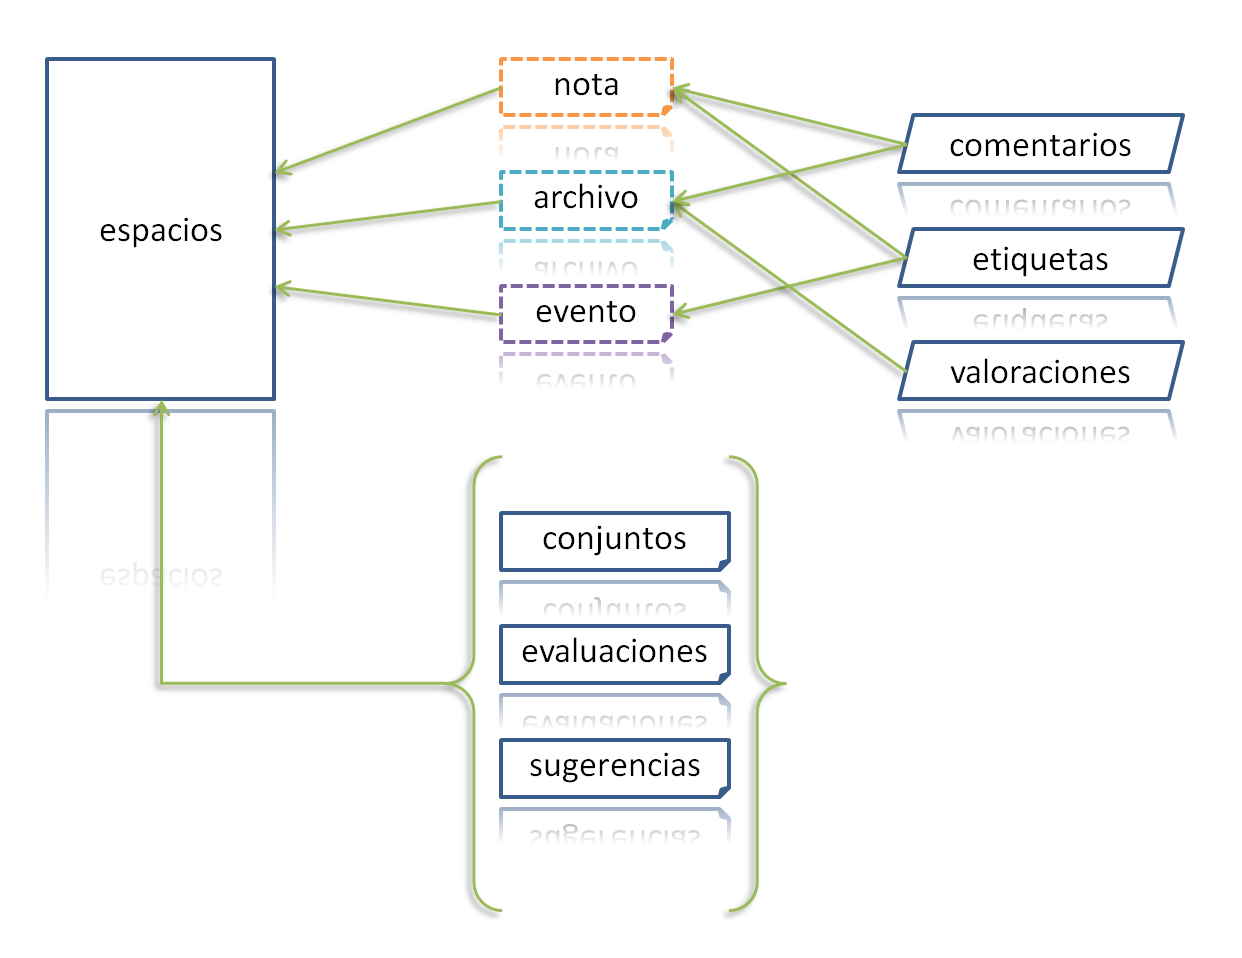
\includegraphics[scale=0.25]{graphics/nomenclatura.png}
 \caption {Relaci\'on entre los conceptos utilizados en el sistema}
 \label {nomenclatura}
\end{figure}

\subsection{Resultados}
Definidos los terminos a utilizarse, a continuaci\'on se present\'an los resultados generados:

\subsubsection{Contexto}
\begin{center}
\begin{tabular}{|l|l|}
\hline
Sitio web & \url{yachay.memi.umss.edu.bo} \\
Periodo acad\'emico & I/2011 \\
Tiempo de evaluaci\'on: & 325 dias. \\
Fecha de inicio: & 23 de Septiembre del 2010. \\
Fecha de fin: & 14 de Agosto del 2011. \\
Lugar de evaluaci\'on: & Carrera de Inform\'atica y Sistemas (UMSS). \\
Ca\'idas del servidor: & 4. \\
Tiempo del servidor fuera de linea: & 2 semanas acumuladas. \\
Docentes participantes: & 4. \\
Materias participantes: & 4. \\
Grupos participantes: & 8. \\
Usuarios participantes: & 542 (estudiantes de primeros semestres). \\
Espacios virtuales creados: & 33. \\
Recursos publicados: & 68. \\
\hline
\end{tabular}
\end{center}
\subsubsection{Usuarios}

En t\'erminos de uso, puede apreciarse en la Figura \ref{usuarios_tabla_1} las diferentes formas de comportamiento de los 
usuarios, seg\'un el rol que desempe\~nan en el sistema.
Destaca en esta tabla la disparidad entre el rol de estudiante y los dem\'as roles, como puede verse en la Figura 
\ref{usuarios_bars_1}, del conjunto de usuarios registrados, \'unicamente el 20\% ingreso alguna vez al sistema,
Es de rescatar adem\'as, que los usuarios fueron registrados autom\'aticamente por sus respectivos docentes.

\begin{figure}[H]
\centering
 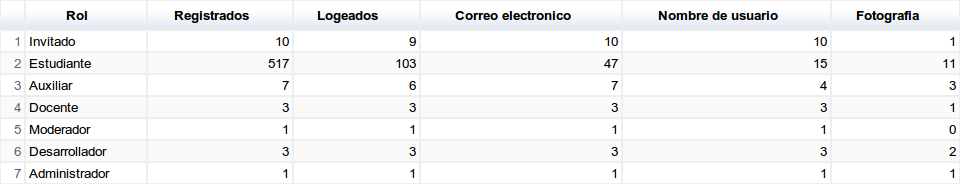
\includegraphics[scale=0.4]{graphics/usuarios_tabla_1.png}
 \caption {Intenci\'on de los usuarios clasificados por rol}
 \label {usuarios_tabla_1}
\end{figure}

\begin{figure}[H]
\centering
 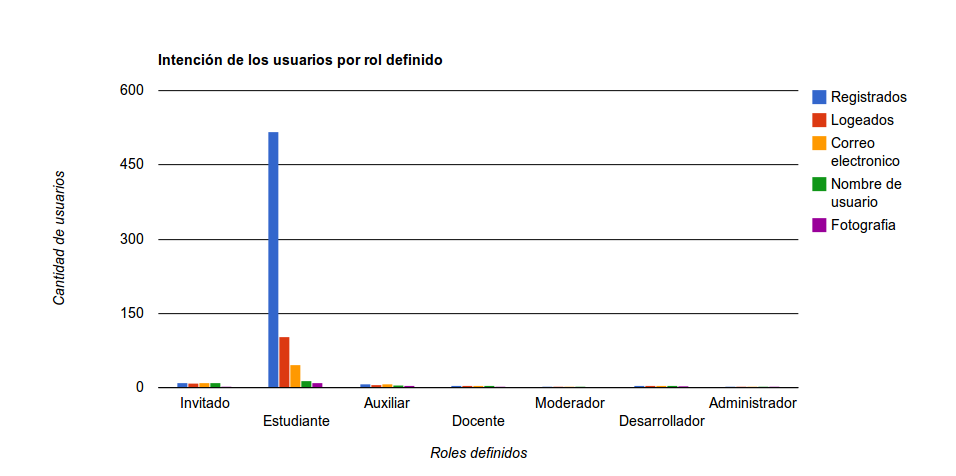
\includegraphics[scale=0.4]{graphics/usuarios_bars_1.png}
 \caption {Diagrama de barras de la intenci\'on de los usuarios clasificados por rol}
 \label {usuarios_bars_1}
\end{figure}

Puede verse en la Figura \ref{usuarios_pie_1} como el predominio en cantidad de los estudiantes va decayendo progresivamente
en intenci\'on frente a los otros roles. Considerando los escasa cantidad de atractivos que posee el sistema es importante 
considerar una audiencia de 126 personas como el primer paso hacia la construcci\'on de un lugar com\'un para el estudio 
realizado.\\

Respecto a la actividad de los usuarios sobre el sistema, puede verse en la Figura \ref{usuarios_tabla_2} la escasisima 
actividad, participaci\'on y popularidad en todos los roles, exceptuando el de los desarrolladores. Puede verse tambi\'en en
la Figura \ref{usuarios_bars_2} el prometedor indicador de sociabilidad, que como puede verse en la Figura 
\ref{usuarios_pie_2} es el mas homog\'eneo, lo que augura una conectividad mas que deseable para los usuarios.

\begin{figure}[H]
\centering
 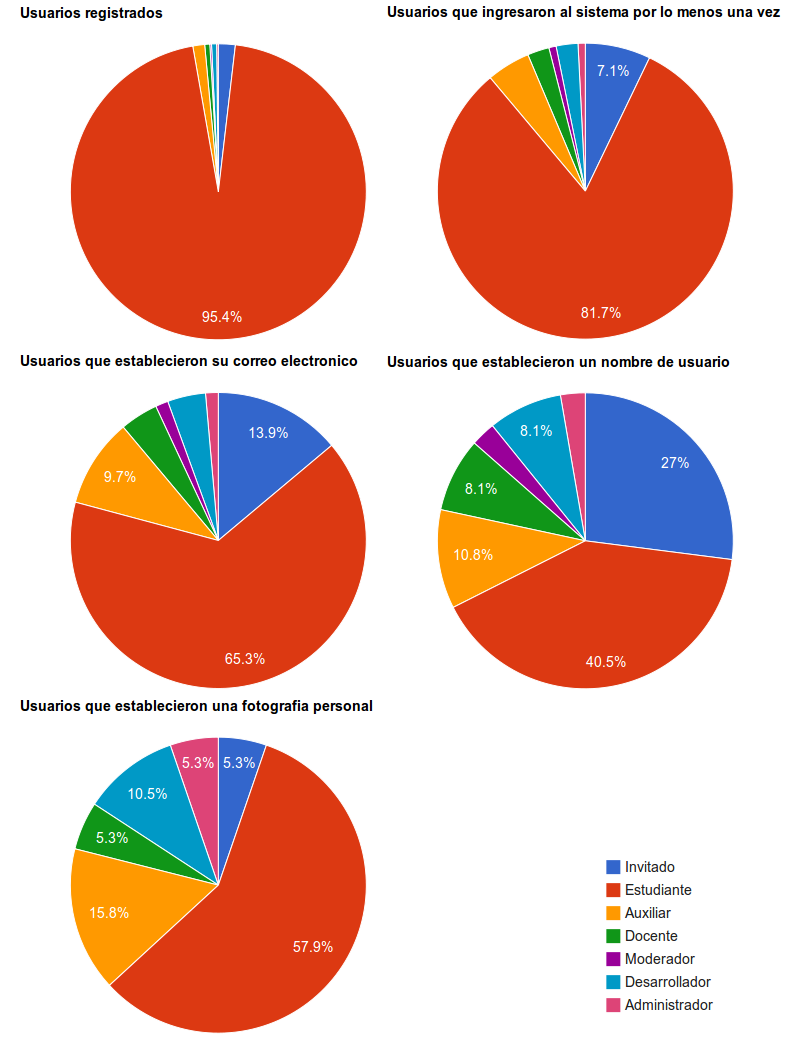
\includegraphics[scale=0.4]{graphics/usuarios_pie_1.png}
 \caption {Porcentajes de intenci\'on de los usuarios clasificados por rol}
 \label{usuarios_pie_1}
\end{figure}

\begin{figure}[H]
\centering
 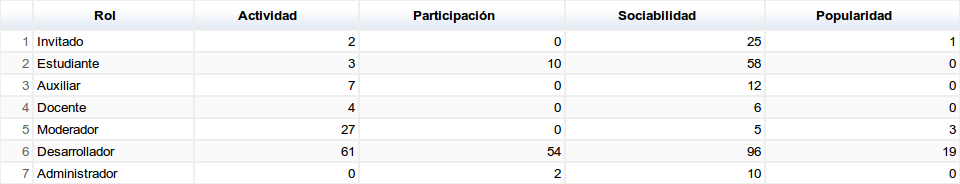
\includegraphics[scale=0.4]{graphics/usuarios_tabla_2.png}
 \caption {Actividad de los usuarios clasificados por rol}
 \label {usuarios_tabla_2}
\end{figure}

\begin{figure}[H]
\centering
 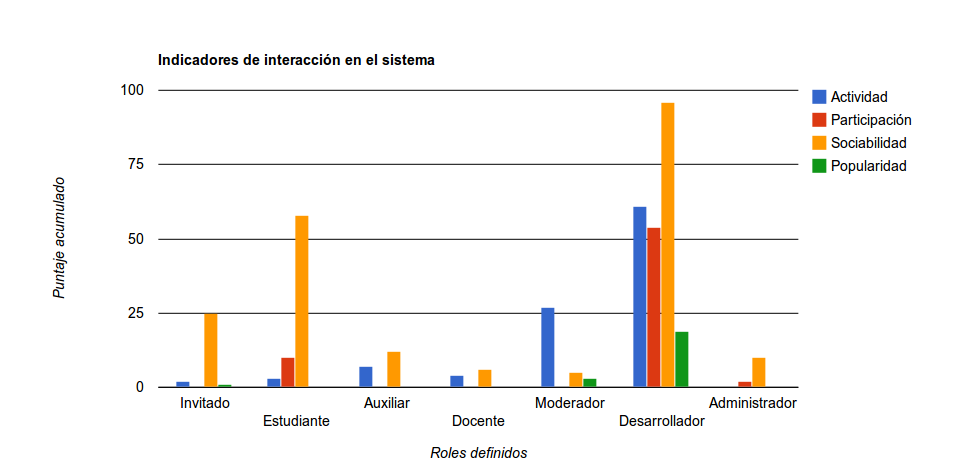
\includegraphics[scale=0.4]{graphics/usuarios_bars_2.png}
 \caption {Diagrama de barras de la actividad de los usuarios clasificados por rol}
 \label {usuarios_bars_2}
\end{figure}

\begin{figure}[H]
\centering
    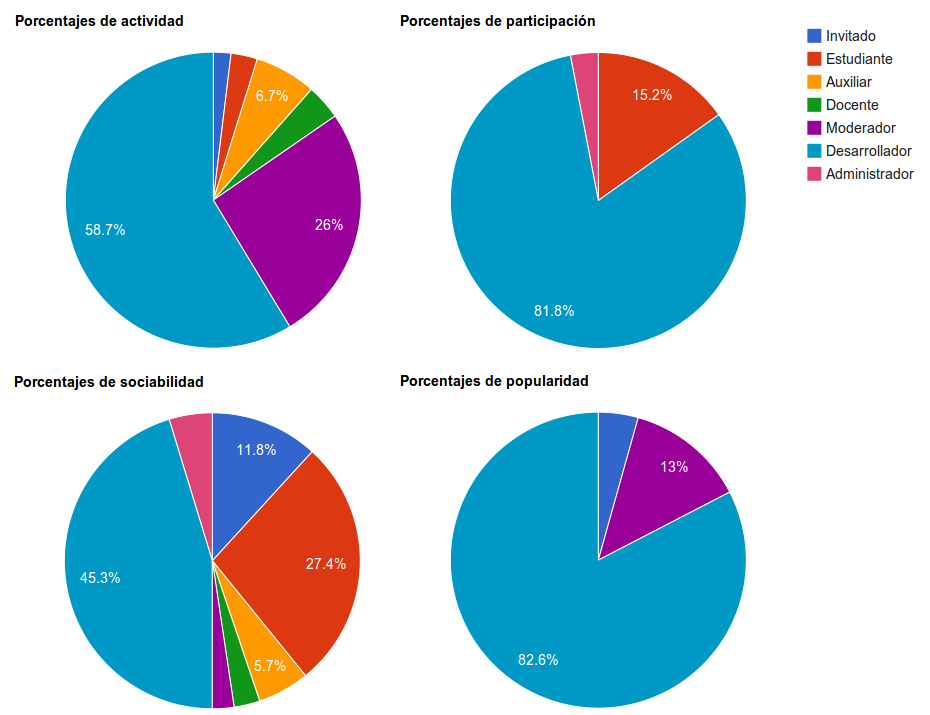
\includegraphics[scale=0.4]{graphics/usuarios_pie_2.png}
    \caption {Porcentajes de actividad clasificados por rol}
    \label {usuarios_pie_2}
\end{figure}

\subsubsection{Contactos}

Considerando los indicadores de sociabilidad, puede apreciarse la matriz de adyacencias (Figura \ref{contactos_matriz}) de la
red social, puede verse que los enlaces fuertes son casi exclusividad propia de los desarrolladores, siendo entre
los otros roles predominantes los enlaces d\'ebiles. Puede verse tambi\'en una sutil relaci\'on entre los usuarios que 
establecieron el nombre de usuario en su perfil, y los niveles de sociabilidad. Cuya interrelaci\'on, es motivo
de seguimiento e intenci\'on de demostraci\'on.
\begin{figure}[H]
\centering
    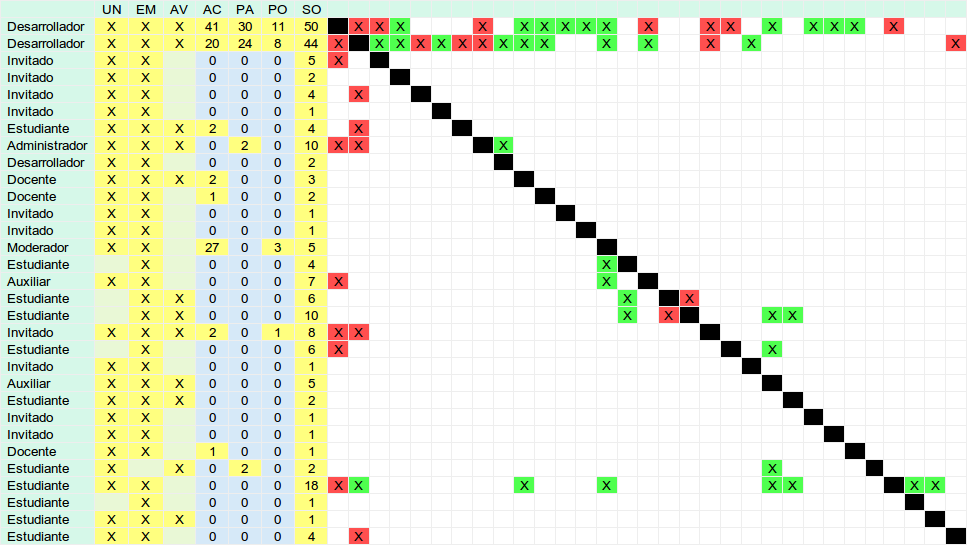
\includegraphics[scale=0.4]{graphics/contactos_matriz.png}
    \caption {Matriz de adyacencia de la red social}
    \label {contactos_matriz}
\end{figure}

\subsubsection{Espacios Virtuales}

En la Figura \ref{espacios_tabla_1} pueden verse los distintos tipos de espacios virtuales y sus indicadores propios, entre 
los que destaca la supremac\'ia del espacio portada, por sobre cualquier otro espacio, siendo el que 
capta mas audiencia de entre los espacios. Tambi\'en es notorio el ausente uso de espacios para equipos de trabajo en los 
grupos, cosa que puede ser debida a las escasez de grupos registrados. Si bien la portada acapara la 
mayor audiencia, no acapara la mayor cantidad de recursos (Figura \ref{espacios_bars_1}), llev\'andose los espacios de 
comunidades un 45\% del contenido del sitio, reforzando la teor\'ia de fomento hacia los espacios menos 
formales (Figura \ref{espacios_pie_1}).
\begin{figure}[H]
\centering
    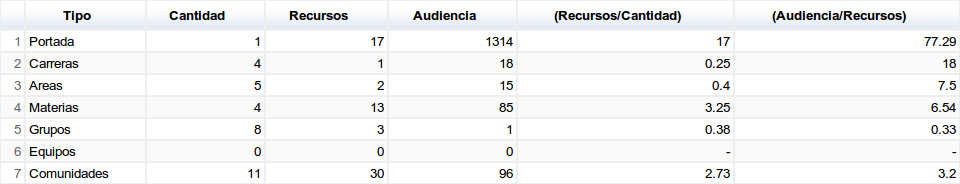
\includegraphics[scale=0.4]{graphics/espacios_tabla_1.png}
    \caption {Clasificaci\'on de los espacios y su actividad}
    \label {espacios_tabla_1}
\end{figure}

\begin{figure}[H]
\centering
    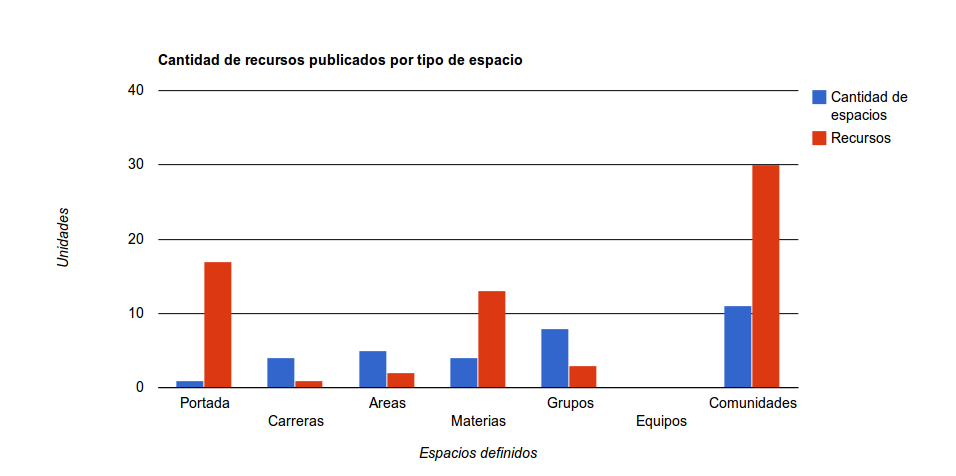
\includegraphics[scale=0.4]{graphics/espacios_bars_1.png}
    \caption {Diagrama de barras de los espacios y sus recursos}
    \label {espacios_bars_1}
\end{figure}

\begin{figure}[H]
\centering
    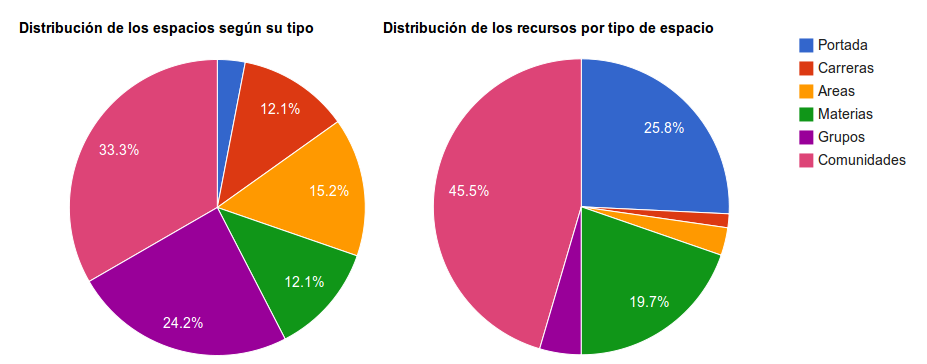
\includegraphics[scale=0.4]{graphics/espacios_pie_1.png}
    \caption {Porcentajes de los espacios y sus recursos seg\'un su tipo}
    \label {espacios_pie_1}
\end{figure}

\subsubsection{Recursos}

Los recursos pueden ser de varios tipos (Figura \ref{recursos_tabla_1}), destacando la gran cantidad de notas 
(Figura \ref{recursos_bars_1}) por sobre los otros tipos de recursos, pudiendo esto deberse a la inmensa facilidad de 
creaci\'on de estas. Aun asi son las fotograf\'ias la que en proporci\'on reciben mejor audiencia, y son los archivos los 
que reciben mayor cantidad de comentarios (Figura \ref{recursos_pie_1}).
\begin{figure}[H]
\centering
    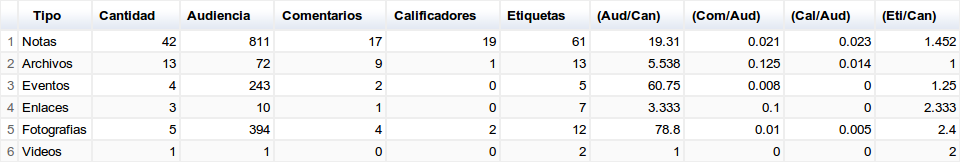
\includegraphics[scale=0.4]{graphics/recursos_tabla_1.png}
    \caption {Clasificaci\'on de los recursos seg\'un su tipo}
    \label {recursos_tabla_1}
\end{figure}

\begin{figure}[H]
\centering
    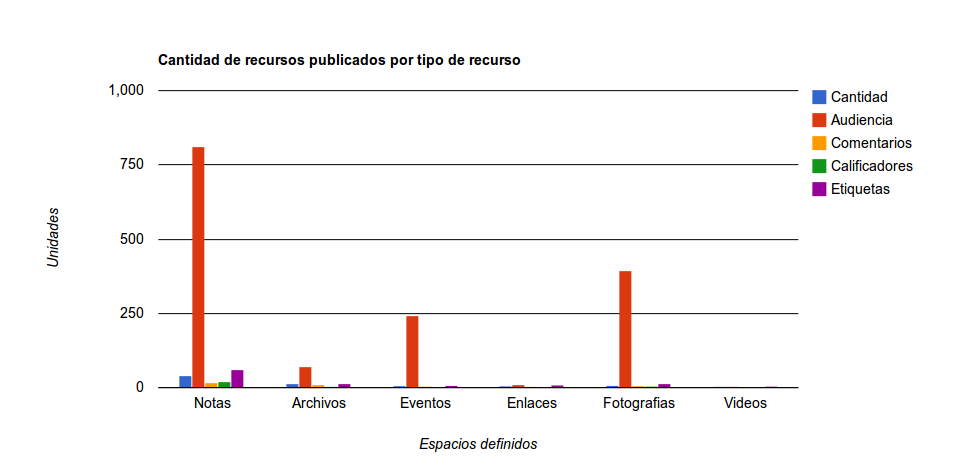
\includegraphics[scale=0.4]{graphics/recursos_bars_1.png}
    \caption {Diagrama de barras de los recursos y sus niveles de repercusi\'on}
    \label {recursos_bars_1}
\end{figure}

\begin{figure}[H]
\centering
    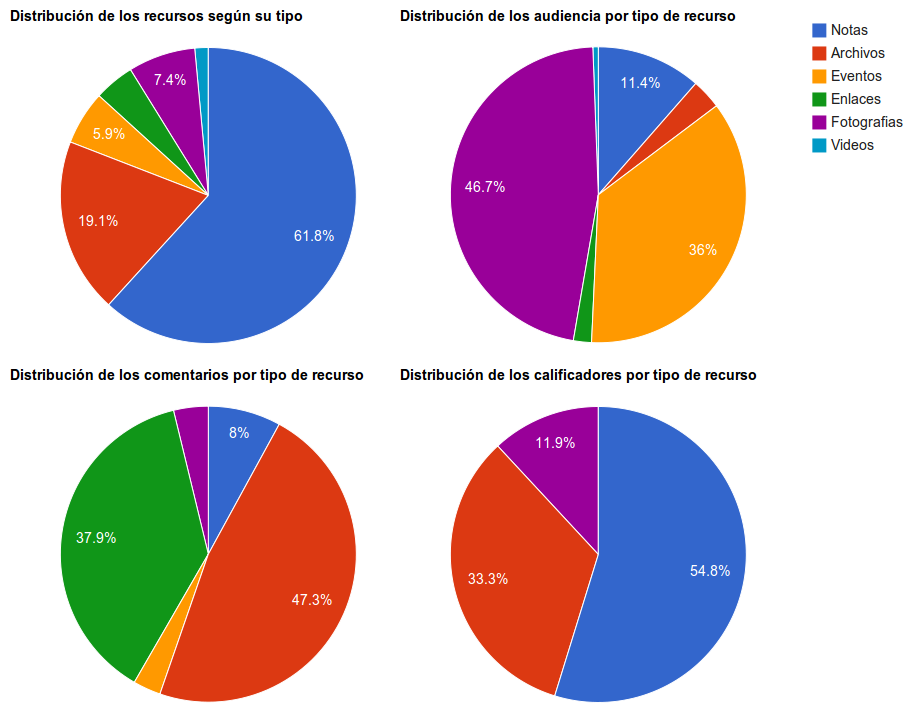
\includegraphics[scale=0.4]{graphics/recursos_pie_1.png}
    \caption {Porcentajes de los recursos seg\'un su tipo}
    \label {recursos_pie_1}
\end{figure}

\subsubsection{Linea de tiempo}

Finalizados los elementos propios de la herramienta, se observan ahora las lineas de tiempo, donde se presentan los tiempos
en los que estos elementos han sido creados.
En la Figura \ref{tiempos_area_1} puede apreciarse en la linea de creaci\'on de los usuarios, los registros autom\'aticos de 
los estudiantes, de parte del docente de su materia, siendo la creaci\'on de usuarios la linea predominante en esta gr\'afica.
\begin{figure}[H]
    \centering
    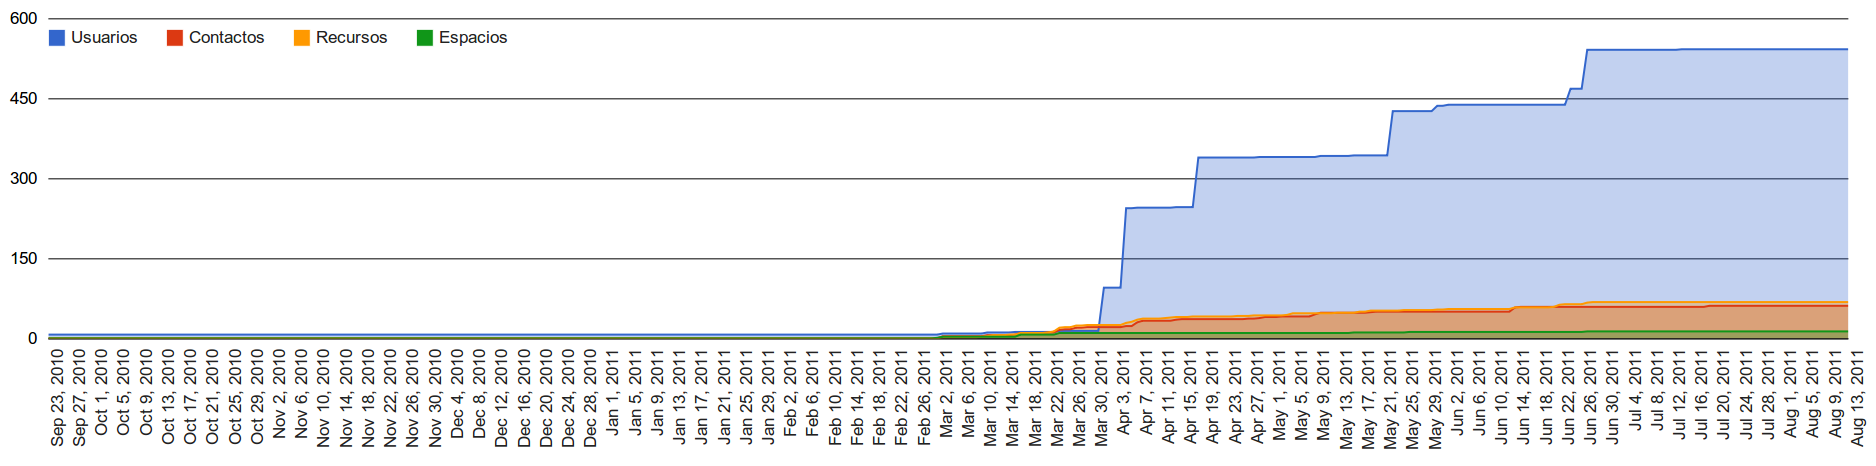
\includegraphics[scale=0.25]{graphics/tiempos_area_1.png}
    \caption {Linea de tiempo de la creaci\'on de elementos en el sistema}
    \label {tiempos_area_1}
\end{figure}

En la Figura \ref{tiempos_area_2} resalta la curiosa relaci\'on entre las lineas de creaci\'on de recursos y la de creaci\'on
de contactos, siendo esta la linea que determina todo el objeto de investigaci\'on.
\begin{figure}[H]
\centering
    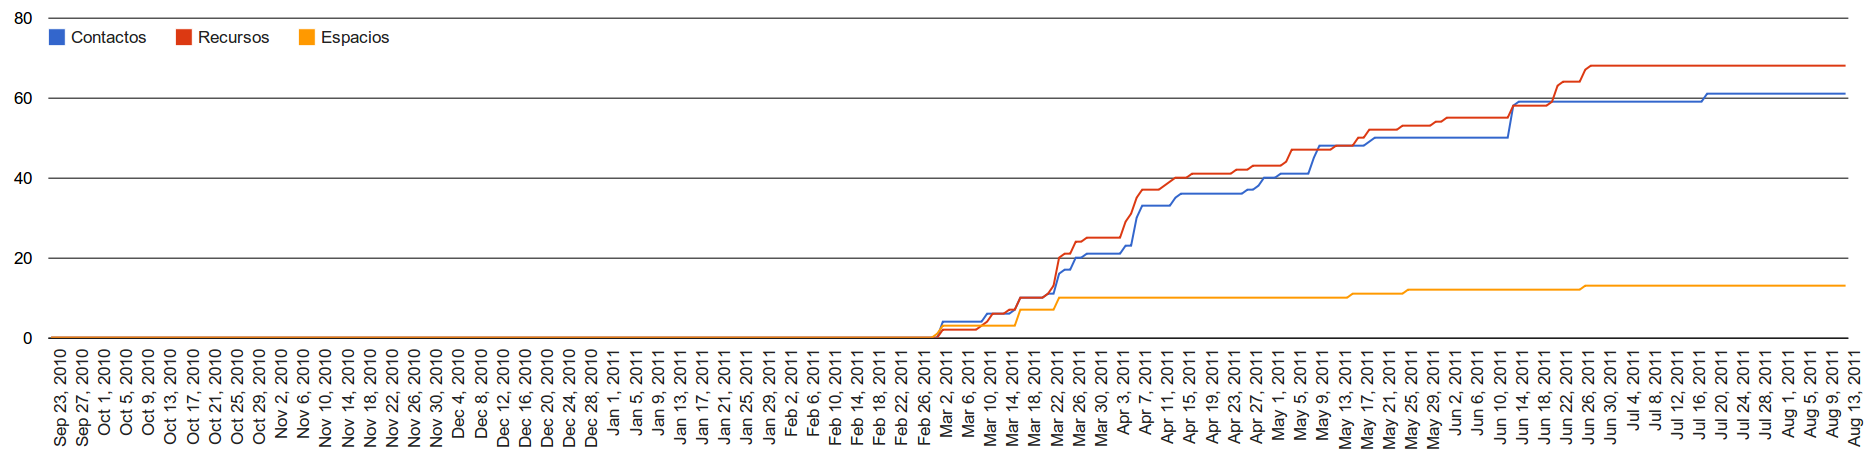
\includegraphics[scale=0.25]{graphics/tiempos_area_2.png}
    \caption {Linea de tiempo de la creaci\'on de elementos en el sistema}
    \label {tiempos_area_2}
\end{figure}

